\documentclass[12pt]{article}
\usepackage{bm}
\usepackage{graphicx}
\usepackage{gensymb}
\graphicspath{{./../images/}}

\begin{titlepage}

\title{\textbf{Optimum Loft Angle for Greatest Carry Distance}}
\author{\textbf{Group D}\\
		Alison McIntosh\\
		Emily Dark\\
		Henry Archer\\
		Kyle Stewart\\
		Stuart Ballantyne}
\date{}

\end{titlepage}

\begin{document}

\begin{titlepage}
\maketitle
\thispagestyle{empty}
\pagebreak
\end{titlepage}

\pagenumbering{arabic}

\section{Abstract}
...


\section{Response}
...

\section{Theory and model}

\subsection{Assumptions}
The following assumptions are made throughout the report and model:
\begin{description}
  \item[$\cdot$] golf course is level and has no effect on trajectory;
  \item[$\cdot$] height of the tee is negligible;
  \item[$\cdot$] gravitational field strength is constant (9.81 $N\cdot kg^{-1}$) and does not flucuate with height;
  \item[$\cdot$] driver is roughly a flat plate and strikes the ball precisely at the center, with no draw or fade.
\end{description}

\subsection{Impact}
...
\pagebreak
\subsection{Flight}
\subsubsection{Simple golf ball}
A simple golf ball experiencing only weight may be modelled with the following system of differential equations;
\begin{equation}
\frac{\partial v_x}{\partial t}=0
\end{equation}
\begin{equation}
\frac{\partial v_y}{\partial t}=-g
\end{equation}
where $g$ is the gravitional field strength.

\begin{figure}[h]
\caption{Golf ball trajectory under no air resistance or lift}
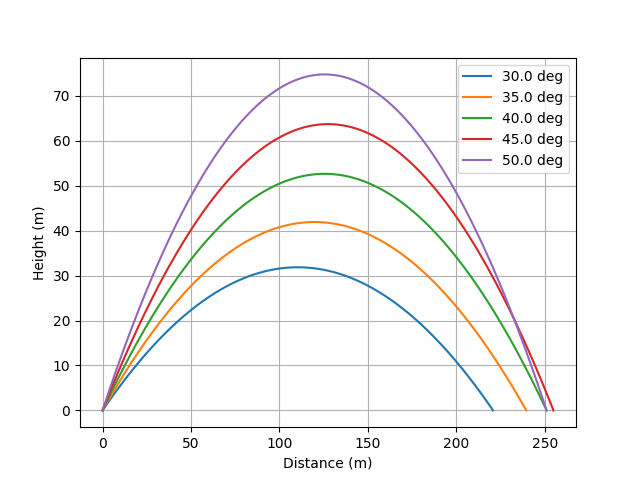
\includegraphics[scale=0.8]{simple}
\end{figure}

Figure 1 shows the maximum range is when the loft angle is 45\degree as predicted by projectile motion equations.

\subsubsection{Smooth golf ball experiencing drag}
The drag equation is;
\begin{equation}
F_d = \frac{1}{2} A C_d \rho_{air} |\vec{v}| \vec{v}
\end{equation}
where $\rho_{air}$ is the density of air; $A$ is the reference area, which in the case of a smooth sphere of radius $r$, is the cross-sectional area $\pi r^2$; $C_d$ is the coefficient of drag, which is dependent on the Reynolds number; and $\vec{v}$ is the velocity vector of the golf ball.


\begin{figure}[h]
\caption{Golf ball trajectory when experiencing drag but no lift}
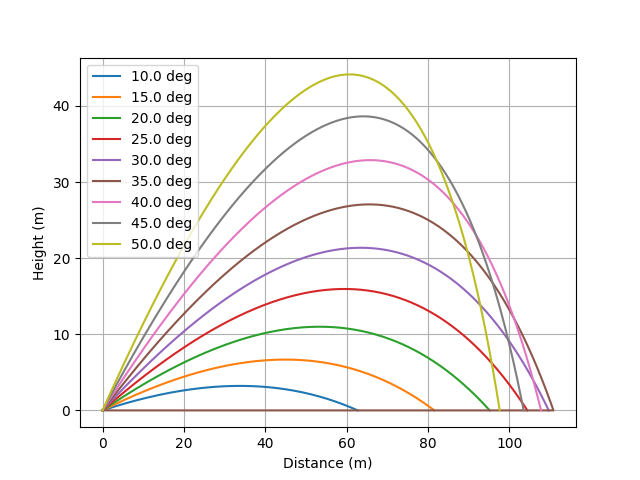
\includegraphics[scale=0.8]{drag}
\end{figure}

\end{document}
\grid